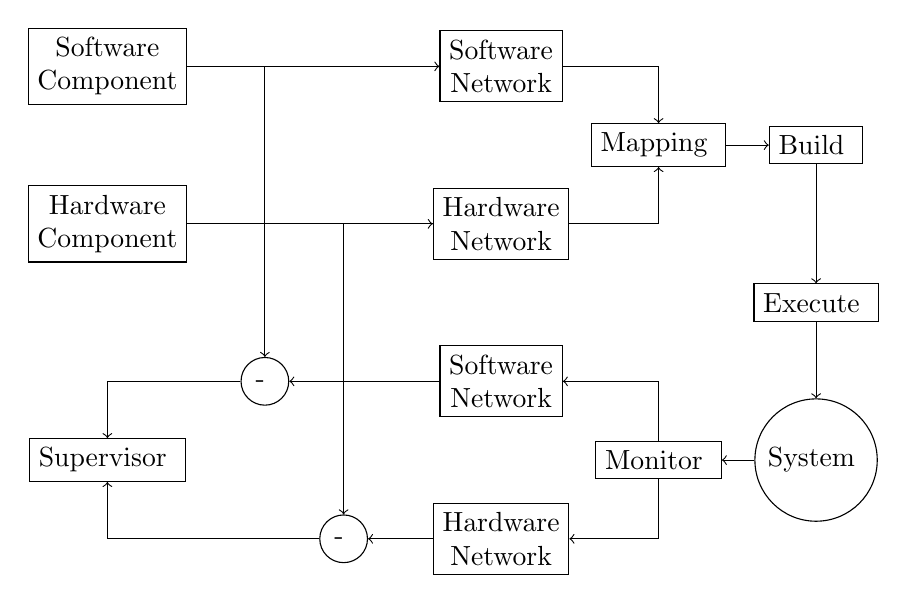
\begin{tikzpicture}
        \node[draw, align=center] (SWCOMP) at (0,1) {
            Software\\Component
        };
        \node[draw, align=center] (HWCOMP) at (0,-1) {
            Hardware\\Component
        };
        \node[draw, align=center] (SWNET) at (5,1) {
            Software\\Network
        };
        \node[draw, align=center] (HWNET) at (5,-1) {
            Hardware\\Network
        };
        \node[draw, align=center] (MAP) at (7,0) {
            Mapping
        };
        \node[draw, align=center] (BUILD) at (9,0) {
            Build
        };
        \node[draw, align=center] (EXEC) at (9,-2) {
            Execute
        };
        \node[circle, draw, align=center] (SYS) at (9,-4) {
            System
        };
        \node[draw, align=center] (MON) at (7,-4) {
            Monitor
        };
        \node[draw, align=center] (SWNET2) at (5,-3) {
            Software\\Network
        };
        \node[draw, align=center] (HWNET2) at (5,-5) {
            Hardware\\Network
        };
        \node[circle, draw, align=center] (SWDIFF) at (2,-3) {
            -
        };
        \node[circle, draw, align=center] (HWDIFF) at (3,-5) {
            -
        };
        \node[draw, align=center] (SUPERVISOR) at (0,-4) {
            Supervisor
        };
        \draw[->] (SWNET) -| (MAP);
        \draw[->] (HWNET) -| (MAP);
        \draw[->] (MAP) -- (BUILD);
        \draw[->] (BUILD) -- (EXEC);
        \draw[->] (EXEC) -- (SYS);
        \draw[->] (SYS) -- (MON);
        \draw[->] (MON) |- (SWNET2);
        \draw[->] (MON) |- (HWNET2);
        \draw[->] (SWNET) -| (SWDIFF);
        \draw[->] (SWNET2) -- (SWDIFF);
        \draw[->] (HWNET) -| (HWDIFF);
        \draw[->] (HWNET2) -- (HWDIFF);
        \draw[->] (SWDIFF) -| (SUPERVISOR);
        \draw[->] (HWDIFF) -| (SUPERVISOR);
        \draw[->] (SWCOMP) -- (SWNET);
        \draw[->] (HWCOMP) -- (HWNET);
\end{tikzpicture}
